\documentclass[14pt, oneside]{altsu-bachelor}

\title{Сервис автоматизированного решения CAPTCHA}
\author{А.\,В.~Лаптев}
\groupnumber{5.306M}
\GradebookNumber{1337}
\supervisor{В.\,В.~Электроник}
\supervisordegree{к.ф.-м.н., доцент}
\ministry{Министерство науки и высшего образования}
\country{Российской Федерации}
\fulluniversityname{ФГБОУ ВО Алтайский государственный университет}
\institute{Институт цифровых технологий, электроники и физики}
\department{Кафедра вычислительной техники и электроники}
\departmentchief{В.\,В.~Пашнев}
\departmentchiefdegree{к.ф.-м.н., доцент}
\shortdepartment{ВТиЭ}
\ChairmanOfTheStateCertificationCommission{С.\,П.~Пронин}
\ChairmanOfTheStateCertificationCommissiondegree{д.т.н., проф.}
\NormController{А.\,В.~Калачёв}
\NormControllerdegree{к.ф.-м.н., доцент}
\Consultant{}
\Consultantdegree{}
\UDC{004.94}
\docname{БР 09.03.01}
\abstractRU{Объём текста не менее 1000 символов! Пока счётчики выставляются в ручную, при необходимости правьте cls-файл.}
\abstractEN{Большой текст на английском!}
\keysRU{компьютерное моделирование, cистема управления версиями}
\keysEN{computer simulation, distributed version control}
\countWorkPage{22}
\countWorkImg{6}
\countWorkLit{5}
\countWorkTab{6}

\date{\the\year}

% Подключение файлов с библиотекой.
\addbibresource{graduate-students.bib}

\begin{document}
\maketitle

\setcounter{page}{2}
\makeabstract
\tableofcontents

\chapter{Теоретические основы и эволюция технологии CAPTCHA}

\section{Происхождение и функциональное назначение CAPTCHA}

Проверочный код CAPTCHA (Completely Automated Public Turing test to tell Computers 
and Humans Apart) -- это метод защиты, основанный на принципе аутентификации 
<<вызов-ответ>>. Он предназначен для предотвращения автоматических действий, таких 
как спам или попытки взлома учетных записей, путем выполнения пользователем 
простого теста, подтверждающего, что он человек, а не программа~\cite{support}. 
Термин был придуман в 2003 году~\cite{captcha2003}.

Исторически распространенный тип CAPTCHA был впервые изобретен в 1997 году двумя 
группами, работающими параллельно. Эта форма CAPTCHA требует ввода 
последовательности букв или цифр из искаженного изображения. Поскольку тест 
проводится компьютером, в отличие от стандартного теста Тьюринга, который 
проводится человеком, CAPTCHA иногда описываются как обратные тесты Тьюринга
~\cite{reversecaptcha}.

Набравшая популярность технология reCAPTCHA, была приобретена Google в 2009 году
~\cite{googlerecaptcha}. В дополнение к предотвращению мошенничества с ботами для 
пользователей, Google использовал технологию reCAPTCHA для оцифровки архивов The 
New York Times и книг из Google Books в 2011 году~\cite{nytimes}.

На сегодняшний день CAPTCHA является важной мерой безопасности, так как 
предотвращает автоматические атаки, например, массовую регистрацию ботов, и 
защищает данные пользователя. Современные системы CAPTCHA используют не только 
текст, но и изображения, аудио, поведенческие анализы и другие инновационные 
подходы, чтобы сделать тесты удобными для людей, но сложными для программ. 
Среднестатистическому человеку требуется около 10 секунд, чтобы решить типичный 
CAPTCHA.

\section{Типология CAPTCHA по формату взаимодействия с пользователем}

На сегодняшний день наиболее распространенные виды CAPTCHA включают:

\begin{enumerate}
    \item reCAPTCHA -- разработанная Google система, которая предлагает тесты 
    на основе распознавания объектов, анализа поведения или текстовых символов.
    \item hCAPTCHA -- альтернатива reCAPTCHA, фокусирующаяся на защите 
    конфиденциальности пользователей.
    \item Capy -- система CAPTCHA, предлагающая пользователю головоломки, 
    например, сборку изображения или взаимодействие с элементами интерфейса
    ~\cite{tproger}.
\end{enumerate}

reCAPTCHA -- система защиты от автоматизированных действий, разработанная Google, 
которая помогает различать человека и бота. Она объединяет несколько подходов, 
делая проверку удобной для пользователей, но сложной для автоматических систем.

reCAPTCHA включает в себя следующие версии~\cite{recaptchaversions}:

\begin{enumerate}
    \item reCAPTCHA v1 (устарела в 2018 году):
    \begin{enumerate}
        \item пользователи вводили текст, состоящий из искаженных слов, 
        отображаемых на изображении;
        \item использовала слова из книг и документов, которые не могли быть 
        распознаны OCR.
    \end{enumerate}
    \item reCAPTCHA v2:
    \begin{enumerate}
        \item клик по флажку: пользователи подтверждают, что они не роботы, 
        нажимая на флажок «Я не робот»;
        \item выбор объектов на изображениях: пользователи идентифицируют 
        заданные объекты на сетке из картинок;
        \item аудио CAPTCHA: для пользователей с ограничениями зрения, 
        предлагается прослушать запись и ввести услышанные символы.
    \end{enumerate}
    \item reCAPTCHA v3:
    \begin{enumerate}
        \item полностью работает в фоновом режиме, анализируя поведение 
        пользователя на странице;
        \item не требует явных действий, если пользователь считается 
        низкорискованным~\cite{recaptchaversions}.
    \end{enumerate}
\end{enumerate}

hCAPTCHA -- это альтернативная система CAPTCHA, разработанная для защиты сайтов 
от ботов и спама, при этом уделяющая особое внимание конфиденциальности 
пользователей. Она стала популярной благодаря своей гибкости и ориентации на 
защиту данных~\cite{hcaptcha}.  

Основные особенности hCAPTCHA:

\begin{enumerate}
    \item конфиденциальность:
    \begin{enumerate}
        \item в отличие от reCAPTCHA, hCAPTCHA не собирает данные о 
        пользователях для рекламных целей, что делает ее привлекательной с точки 
        зрения соблюдения конфиденциальности.
    \end{enumerate}
    \item простота интеграции:
    \begin{enumerate}
        \item легко интегрируется с web-сайтами через API;
        \item совместима с большинством популярных платформ, таких как WordPress, 
        и может быть настроена для разных типов взаимодействия.
    \end{enumerate}
    \item модели монетизации:
    \begin{enumerate}
        \item владельцы сайтов могут зарабатывать, разрешая hCAPTCHA 
        использовать проверочные задачи, связанные с машинным обучением, 
        например, разметку данных.
    \end{enumerate}
\end{enumerate}

Виды взаимодействия с пользователями:

\begin{enumerate}
    \item графическая CAPTCHA: выбор изображений, соответствующих запросу;
    \item текстовая CAPTCHA: ввод символов (редко используется);
    \item аудио CAPTCHA: для пользователей с ограниченными возможностями, 
    предлагается прослушать и ввести услышанные символы;
    \item клик CAPTCHA: нажатие на флажок «Я не робот» (для низкорискованных 
    пользователей).
\end{enumerate}

Capy CAPTCHA -- это инновационная система CAPTCHA, разработанная с акцентом на 
удобство для пользователей и адаптацию к современным web-средам. Она предлагает 
интерактивные методы проверки, направленные на минимизацию раздражения 
пользователей при сохранении высокого уровня защиты от ботов~\cite{capy}.

Основные особенности Capy CAPTCHA:

\begin{enumerate}
    \item интерактивность:
    \begin{enumerate}
        \item Capy использует методы проверки, которые требуют не просто ввода 
        текста или выбора картинок, а выполнения задач, таких как перемещение 
        объектов;
        \item простые задачи делают процесс проверки менее раздражающим и более 
        интуитивным;
    \end{enumerate}
    \item гибкость настройки:
    \begin{enumerate}
        \item система может быть адаптирована под конкретные нужды сайта, 
        включая выбор сложности задач и дизайн интерфейса.
    \end{enumerate}
    \item доступность:
    \begin{enumerate}
        \item подходит для пользователей с различными потребностями, включая 
        мобильные устройства.
    \end{enumerate}
\end{enumerate}

Виды взаимодействия с пользователями:

\begin{enumerate}
    \item головоломки (Puzzle CAPTCHA): сборка пазла с перемещением недостающих 
    элементов в нужное место;
    \item тесты на логику и распознавание: выбор нужного объекта или 
    логического варианта из предложенных;
    \item текстовая CAPTCHA (редко используется).
\end{enumerate}

Capy CAPTCHA используется на сайтах, где важны как защита от ботов, так и 
положительный пользовательский опыт. Особенно популярна в проектах с высоким 
акцентом на дизайн и пользовательское взаимодействие.

\section{Критерии надежности и уязвимости различных CAPTCHA-систем}

Эффективность CAPTCHA-систем определяется совокупностью признаков. К основным 
критериям надежности относятся~\cite{captchawiki}:

\begin{enumerate}
    \item устойчивость к машинному распознаванию, в том числе с использованием 
    современных алгоритмов искусственного интеллекта;
    \item наличие разнообразных и уникальных тестов, исключающих возможность 
    формирования обучающих или атакующих датасетов;
    \item доступность и понятность графического пользовательского интерфейса для 
    широкой аудитории.
\end{enumerate}

Несмотря на свою популярность, CAPTCHA-системы обладают рядом уязвимостей, 
снижающих их надежность и ухудшающих пользовательский опыт~\cite{captchatrouble, 
captchatrouble2}:

\begin{enumerate}
    \item высокая когнитивная нагрузка, связанная со сложностью задач для 
    человека;
    \item недоступность или трудности прохождения для отдельных групп 
    пользователей, включая людей с нарушениями зрения или слуха;
    \item низкая эффективность против целевых атак или сервисов, управляемых 
    человеком;
    \item несовместимость с некоторыми web-браузерами и мобильными устройствами;
    \item ограниченная поддержка вспомогательных технологий, используемых людьми 
    с ограниченными возможностями.
\end{enumerate}

Для CAPTCHA в текстовом формате выделяют следующие критерии надежности:

\begin{enumerate}
    \item преднамеренное искажение символов (геометрическая деформация, 
    перекрытие, наклоны);
    \item использование нестандартных шрифтов, графических помех и шумов;
    \item отсутствие четкой сегментации между символами, затрудняющей их 
    раздельное распознавание;
    \item рандомизация длины строк и набора используемых символов.
\end{enumerate}

Несмотря на совокупность методов для усложнения автоматизированного 
распознавания, текстовые CAPTCHA подвержены следующим уязвимостям:

\begin{enumerate}
    \item современные OCR-системы и seq2seq-модели, в том числе архитектуры на 
    основе CNN и RNN, успешно справляются с распознаванием даже при наличии 
    искажений;
    \item упрощенные CAPTCHA без шумов и дополнительных помех могут быть 
    распознаны с высокой точностью даже базовыми алгоритмами;
    \item использование ограниченного и фиксированного алфавита позволяет обучать 
    модели, показывающие высокую точность при распознавании.
\end{enumerate}

Для CAPTCHA в аудиоформате основными характеристиками надежности являются:

\begin{enumerate}
    \item введение фонового шума и аудиоискажений, затрудняющих автоматическую 
    обработку;
    \item использование слов, сходных по звучанию, нестандартных акцентов и 
    синтезированной речи;
    \item наложение голосов, изменение темпа и интонации произношения;
    \item высокая вариативность аудиофайлов.
\end{enumerate}

В то же время современным реализациям аудио CAPTCHA присущи следующие уязвимости:

\begin{enumerate}
    \item преобразование аудио в спектрограммы с последующим анализом с помощью 
    CNN и методов CTC позволяет достигать высокой точности распознавания;
    \item современные модели автоматического распознавания речи успешно решают 
    даже зашумленные аудиозадания;
    \item применение генеративных моделей и других методов предварительной 
    обработки аудио позволяет эффективно устранять шумы, повышая точность 
    распознавания.
\end{enumerate}

К ключевым характеристикам надежности CAPTCHA с изображениями относятся:

\begin{enumerate}
    \item использование изображений из реального мира с вариативными фонами и 
    сценами;
    \item намеренное смещение объектов по положению, углу поворота и масштабу;
    \item включение визуально схожих ложных объектов, усложняющих выбор 
    правильных;
    \item разнообразие типов изображений.
\end{enumerate}

Среди основных уязвимостей графических CAPTCHA можно выделить:

\begin{enumerate}
    \item высокая эффективность современных моделей детектирования объектов 
    (например, YOLOv8, Faster R-CNN) при наличии специализированного обучающего 
    датасета;
    \item возможность автоматизации взаимодействия с CAPTCHA (например, выбор 
    изображений) с использованием скриптов и эмуляторов браузеров;
    \item ограниченность числа классов, используемых в задаче, позволяет быстро 
    обучить модель для решения конкретной CAPTCHA.
\end{enumerate}

\chapter{Парсинг изображений CAPTCHA и их предобработка для создания датасета}

\section{Парсинг реальных CAPTCHA с различных web-ресурсов}

Большинство предобученных моделей компьютерного зрения, таких как YOLOv8, обучены на датасете COCO~\cite{COCO}, содержащем изображения высокого качества с чёткими контурами и однозначной аннотацией объектов. Однако CAPTCHA с изображениями имеют принципиально иные характеристики: они могут включать в себя размытие, наложенные артефакты, искажения, шумы, повторяющиеся элементы и искусственно пониженное разрешение. Всё это снижает эффективность использования стандартных датасетов и моделей, не адаптированных под такие условия.

Для обеспечения высокой точности в задаче автоматического решения CAPTCHA необходимо подготовить собственный набор данных, приближённый к реальным условиям использования. Наиболее эффективным методом является автоматизированный парсинг изображений CAPTCHA, представленных на веб-сайтах, использующих визуальные CAPTCHA-решения, такие как Google reCAPTCHA v2.

Использование реальных CAPTCHA, собранных в автоматическом режиме, имеет ряд преимуществ по сравнению с синтетической генерацией данных:

\begin{enumerate}
    \item изображения содержат разнообразные сцены, освещение, углы обзора и уровни шума, что положительно влияет на способность модели к обобщению;
    \item присутствует большое количество уникальных объектов на фоне, в том числе в частично перекрытых и смазанных вариантах;
    \item отсутствует необходимость в ручной генерации изображений и создании дополнительных искажений для повышения реалистичности;
    \item возможно извлекать текстовые инструкции к CAPTCHA, что позволяет соотносить каждое изображение с требуемым классом.
\end{enumerate}

Для парсинга CAPTCHA был реализован автоматизированный сценарий взаимодействия с браузером с использованием библиотеки Selenium~\cite{Selenium}. Данный подход позволяет воспроизвести действия пользователя при работе с CAPTCHA, обходя при этом ручной ввод. Для обеспечения стабильной работы и масштабируемости процесса применялась браузерная автоматизация через WebDriver (в частности, ChromeDriver).

Функциональность парсера включает следующие ключевые этапы:

\begin{enumerate}
    \item поиск iframe-элемента, содержащего чекбокс <<Я не робот>>, и эмуляция клика по нему для инициирования визуальной CAPTCHA;
    \item ожидание загрузки CAPTCHA и извлечение изображения с заданием (включая его URL или пиксельный снимок);
    \item извлечение информации о структуре сетки (количество строк и столбцов), на которую разбито изображение CAPTCHA;
    \item получение текста задания, содержащего имя объекта (например, <<выберите все изображения с мотоциклами>>), для последующего использования в аннотации данных.
\end{enumerate}

Типичная CAPTCHA представляет собой изображение, разделённое на сетку из 3×3 или 4×4 ячеек, каждая из которых может содержать фрагмент сцены. При этом пользователю предлагается выбрать ячейки, в которых присутствует объект заданного класса. Процесс парсинга может быть представлена блок-схемой на рис.~\ref{fig:captcha-flow}.

\begin{figure}[H]
    \centering
    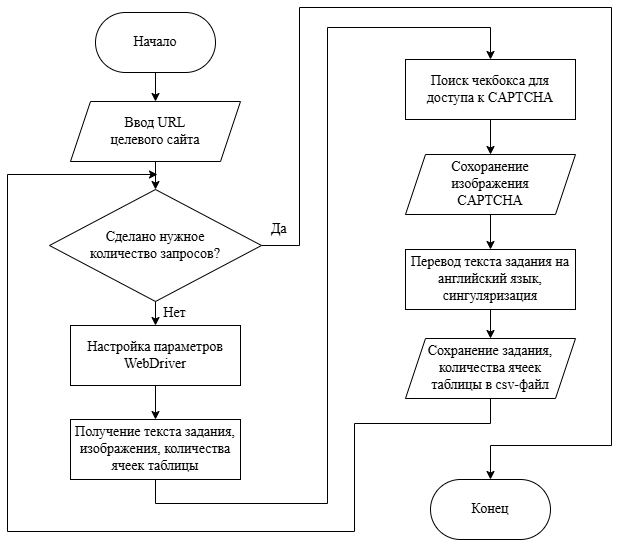
\includegraphics[width=0.65\textwidth]{imgs/image_captcha_flow.png}
    \caption{Блок-схема процесса парсинга CAPTCHA.}
    \label{fig:captcha-flow}
\end{figure}
\vspace{-0.5cm}

Полученные изображения и метаданные (включая текст задания и параметры сетки) используются для формирования обучающего датасета, пригодного для дообучения модели YOLOv8 в задачах классификации и сегментации объектов.

\section{Предварительная обработка изображений датасета}

После получения достаточного количества изображений для составления датасета необходимо провести их предварительную обработку и разметку. Это один из самыхважных этапов работы, поскольку от качества разметки напрямую зависит точность и эффективность последующей работы модели.

Для корректной работы модели YOLO требуется создать иерархическую структуру папок, в которой изображения и соответствующие метки будут разделены на тренировочную и валидационную выборки. Стандартная структура включает следующие директории:

\begin{enumerate}
    \item Директория train -- содержит тренировочную выборку:
    \begin{enumerate}
        \item images -- изображения;
        \item labels -- метки к изображениям.
    \end{enumerate}
    \item Директория val -- содержит валидационную выборку:
    \begin{enumerate}
        \item images -- изображения;
        \item labels -- метки к изображениям.
    \end{enumerate}
\end{enumerate}

Набор классов, пути к выборкам и параметры конфигурации задаются в YAML-файле, который передается при обучении модели. Содержимое такого файла для данной модели:

\begin{code}
\captionof{listing}{\label{code:train-captcha}Параметры конфигурации для обучения модели}
\vspace{-0.5cm}
{\small
\inputminted[mathescape,linenos,frame=lines,breaklines]{yaml}{code/train_captcha.yaml}
}
\end{code}
\vspace{-0.4cm}

Для создания меток используется инструмент CVAT (Computer Vision Annotation Tool) -- многофункциональное веб-приложение с поддержкой аннотации объектов с помощью полигонов, прямоугольников и других форм. CVAT позволяет экспортировать разметку напрямую в формат, совместимый с YOLO~\cite{CVAT}.

Поскольку CAPTCHA-изображения часто содержат объекты с нечёткими контурами, наложением и визуальными искажениями, особенно важно использовать ручную точную разметку, а не ограничиваться автоматическими методами. Выделение объектов должно проводиться как можно точнее, с учётом геометрии контуров. На рисунке ниже представлен пример изображения с размеченными объектами:

\begin{figure}[H]
    \centering
    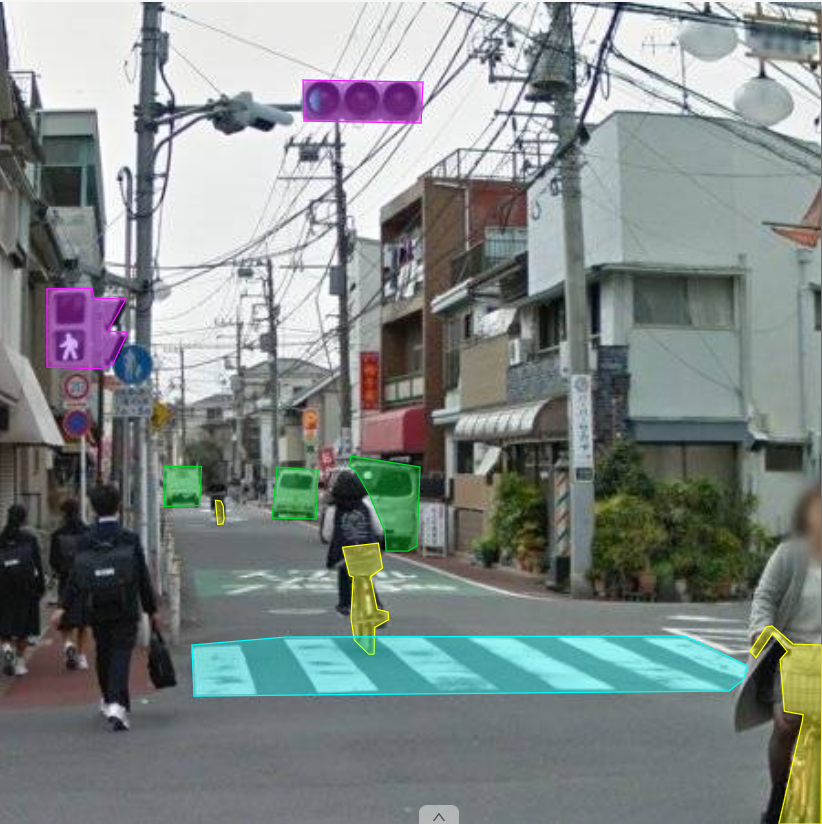
\includegraphics[width=0.9\linewidth]{imgs/captcha-poligons.png}
    \caption{Пример разметки изображения с тестовой CAPTCHA.}
    \label{fig:mask-captcha}
\end{figure}
\vspace{-0.5cm}

Кроме того, разметка позволяет учесть сразу несколько объектов разных классов на одном изображении, что особенно характерно для CAPTCHA, где в одной сетке могут одновременно находиться, например, автомобили и автобусы. Такой подход положительно влияет на обобщающую способность модели.

В случае, если количество данных по отдельным классам окажется недостаточным, можно дополнительно использовать методы аугментации: вращение, масштабирование, искажение цвета и контраста. Однако при хорошо организованном парсинге и разметке зачастую удается обойтись без аугментации.

\chapter{Экспериментальная часть и исследовательский вклад}

\section{Сравнительный анализ моделей нейронных сетей для автоматизированного решения CAPTCHA в текстовом формате}

\textbf{Современная реализация текстовых CAPTCHA}

Современные текстовые CAPTCHA обычно состоят из букв и цифр. Зачастую 
используются символы латинского алфавита (как прописные, так и строчные) и цифры 
от 0 до 9. Но обычно реализации исключают символы, которые могут быть легко 
перепутаны, например, буквы <<O>> и цифру <<0>>, буквы <<I>> и <<l>> и тому 
подобное. Рекомендуемый набор символов в генераторах на некоторых CRM платформах 
выглядит следующим образом: ABCDEFGHJKLMNPQRSTWXYZ23456789~\cite{Bitrix}.

Длина последовательности символов в CAPTCHA обычно составляет от 4 до 8 символов, 
что обеспечивает баланс между удобством для пользователя и безопасностью, однако 
конкретная длина может варьироваться в зависимости от требований системы 
безопасности.

Для усложнения автоматического распознавания текстовые CAPTCHA подвергаются 
различным искажениям:
\begin{enumerate}
    \item геометрические искажения: символы могут быть искажены, повернуты или 
    наклонены, что затрудняет их распознавание автоматическими системами~
    \cite{BrightData};
    \item перекрытие символов: символы могут быть расположены близко друг к 
    другу или даже перекрываться, что усложняет их сегментацию и последующее 
    распознавание~\cite{Proglib};
    \item добавление шума: на изображение могут быть добавлены различные шумы, 
    такие как линии, точки или круги, чтобы затруднить распознавание символов;
    \item сложные фоны: использование фонов с различными цветами или узорами, 
    что делает выделение символов более сложным~\cite{NVJournal};
    \item нелинейные искажения: применение нелинейных трансформаций к символам, 
    что делает их форму менее предсказуемой для автоматических систем 
    распознавания~\cite{Simai}.
\end{enumerate}

Эти методы направлены на повышение сложности автоматического распознавания 
CAPTCHA, сохраняя при этом относительную легкость распознавания для человека. 

\textbf{Подготовка датасета с изображениями и выбор модели нейронной сети}

Качество используемого датасета оказывает существенное влияние на итоговую 
точность работы модели. Для эффективного обучения необходимо, чтобы набор данных 
соответствовал следующим требованиям:

\begin{enumerate}
    \item достаточное количество изображений для каждого символа, что 
    обеспечивает статистическую устойчивость модели;
    \item разнообразие данных, включающее:
    \begin{enumerate}
        \item различные углы наклона символов;
        \item вариативность написания символов и их искажения;
        \item наличие побочных визуальных элементов, создающих препятствия для 
        распознавания;
        \item использование различных шрифтов.
    \end{enumerate}
    \item переменная длина последовательностей символов, что позволяет модели 
    адаптироваться к разным формам CAPTCHA.
\end{enumerate}

Включение указанных факторов способствует обучению модели на более широком 
спектре признаков, что, в свою очередь, повышает её способность к обобщению на 
ранее невидимых данных.

Для распознавания текста с переменной длиной последовательности в задачах CAPTCHA 
наиболее часто применяются следующие архитектуры нейронных сетей:

\begin{enumerate}
    \item оптическое распознавание символов (OCR);
    \item рекуррентные сверточные нейронные сети (CRNN);
    \item архитектуры последовательного обучения (Seq-to-Seq).
\end{enumerate}

С целью выбора наиболее эффективной модели были реализованы и протестированы все 
указанные подходы, после чего была выбрана архитектура, обеспечивающая наилучшую 
точность предсказаний.

Для обучения моделей был сформирован датасет из 100 000 изображений CAPTCHA, 
содержащих случайные последовательности символов длиной от 4 до 7. Такой объем 
данных позволяет добиться высокой обобщающей способности модели и снизить 
вероятность переобучения.

\textbf{Оптическое распознавание символов (OCR Tesseract)}

Изначально предполагалась реализация модели с использованием OCR, поскольку такие 
системы изначально разрабатывались для задач оптического распознавания текста. В 
качестве конкретной модели был выбран Tesseract.

Tesseract является одной из наиболее популярных систем OCR с открытым исходным 
кодом. Tesseract поддерживает более 100 языков, включая сложные письменности~
\cite{Klippa}. В версии 4.0 в модель была интегрирована нейронная сеть на основе 
долговременной краткосрочной памяти (LSTM), что позволило существенно повысить 
точность распознавания, особенно при обработке сложных шрифтов и рукописного 
текста~\cite{GitTesseract}.

Для решения поставленной задачи предполагалось использовать предобученную модель 
Tesseract и дообучить её на специализированном датасете, содержащем изображения 
CAPTCHA с характерными искажениями. Однако в ходе экспериментов было установлено, 
что точность распознавания последовательностей символов целиком составляла 0\%, а 
точность для отдельных символов оказалась крайне низкой. Это связано с тем, что 
архитектура Tesseract недостаточно устойчива к искажениям, характерным для 
CAPTCHA, таким как деформация символов, наложение шумов и изменение углов наклона
~\cite{TrainTesseract}.

Таким образом, было принято решение отказаться от использования Tesseract в 
пользу более адаптированных к данной задаче моделей, таких как сверточные 
рекуррентные нейронные сети (CRNN) или модели последовательного обучения 
(Seq-to-Seq), обладающие высокой устойчивостью к вариативности и искажениям, 
характерным для CAPTCHA.

\textbf{Рекуррентные сверточные нейронные сети (CRNN)}

Сверточно-рекуррентные нейронные сети (CRNN) представляют собой гибридную 
архитектуру, сочетающую в себе возможности сверточных нейронных сетей (CNN) и 
рекуррентных нейронных сетей (RNN). Данный подход используется в задачах, 
связанных с обработкой последовательных данных, таких как распознавание текста, 
речь и видео~\cite{CRNNHabr}.

Основное преимущество CRNN заключается в способности CNN-части извлекать 
пространственные признаки из изображений, тогда как RNN-часть позволяет учитывать 
временные зависимости между последовательными фрагментами данных~\cite{CRNNBook}.

Разработанная модель CRNN для распознавания CAPTCHA включает в себя три ключевых 
блока:
\begin{enumerate}
    \item сверточный блок (CNN): предназначен для выделения признаков из 
    изображений CAPTCHA. Включает в себя три последовательных сверточных слоя, а 
    также методы нормализации и уменьшения размерности признакового пространства;
    \item рекуррентный блок (RNN): использует двунаправленные слои GRU, 
    позволяющие модели учитывать зависимость между последовательными символами в 
    CAPTCHA;
    \item выходной слой: полносвязный, который выполняет классификацию каждого 
    символа в последовательности.
\end{enumerate}

В приложении~\ref{code:crnn} представлена реализация CRNN-модели на языке Python 
с использованием библиотеки TensorFlow/Keras:

В данной архитектуре применяются слои Dropout для регуляризации, также 
используется l2-регуляризация, BatchNormalization для ускорения обучения и 
повышения устойчивости модели, а также функция softmax для предсказания классов 
символов.

После обучения данной модели результаты оказались превосходящими показатели OCR, 
однако все же не достигли удовлетворительного уровня. В частности, точность 
распознавания всей последовательности символов не превышала 10\%, тогда как 
точность классификации отдельных символов составляла около 70\%.

\textbf{Архитектура последовательного обучения (Seq-to-Seq)}

Модели последовательного преобразования (Seq-to-Seq) широко применяются для 
задач, связанных с обработкой последовательностей переменной длины. Они 
используются в таких областях, как машинный перевод, распознавание речи и анализ 
текстов~\cite{Seq2Seq}. Данные модели основаны на архитектуре энкодера-декодера, 
где первый модуль кодирует входную последовательность в скрытое представление, а 
второй декодирует его в выходную последовательность.

Одним из ключевых элементов Seq2Seq является механизм внимания, который позволяет 
декодеру динамически фокусироваться на различных частях входной 
последовательности при генерации выходных символов~\cite{Seq2SeqBook}. Этот 
подход особенно полезен для распознавания CAPTCHA, так как символы в изображениях 
могут иметь разную ориентацию и степень искажения.

Кодировщик, в данной модели принимает входное изображение CAPTCHA и преобразует 
его в компактное представление. Архитектура кодировщика включает:
\begin{enumerate}
    \item четыре сверточных блока, слои пакетной нормализации и слои подвыборки 
    для понижения размерности входных данных;
    \item глобальный усредненный слой для получения векторного представления 
    изображения;
    \item полносвязный слой для финального представления скрытого состояния;
    \item рекуррентный слой для кодирования последовательности, возвращающий 
    последнее скрытое состояние кодировщика.
\end{enumerate}

Декодировщик выполняет пошаговую генерацию выходной последовательности, используя 
скрытое состояние кодировщика. В архитектуру декодировщика входят:
\begin{enumerate}
    \item входной слой для последовательности токенов;
    \item слой вложения, который преобразует входные токены в векторные 
    представления;
    \item рекуррентный слой, обрабатывающий последовательность с учетом скрытого 
    состояния кодировщика;
    \item механизм внимания, который позволяет декодеру учитывать релевантные 
    части входного изображения;
    \item полносвязный слой с функцией активации softmax для предсказания 
    вероятностей символов.
\end{enumerate}

Полная архитектура модели реализована в TensorFlow/Keras и реализация модели 
приведена в приложении~\ref{code:seq2seq}.

На начальных этапах экспериментов предложенная Seq-to-Seq-модель показала 
наилучшие результаты среди рассмотренных вариантов. В отличие от OCR- и 
CRNN-моделей, данная архитектура смогла достичь более высокой точности 
распознавания последовательностей символов, что обусловлено применением 
механизма внимания. Дальнейшая работа с моделью была сосредоточена на её 
оптимизации и улучшении параметров обучения.

\section{Эксперименты по аудио- и графическим CAPTCHA}

\textbf{Выбор языка программирования и инстументов для разработки}

Для разработки сервиса по автоматизации распознавания CAPTCHA был выбран язык 
программирования Python и библиотека для автоматизации тестирования 
web-приложений Selenium.

Python обладает рядом преимуществ для решения подобных задач:

\begin{enumerate}
    \item простота и читаемость кода: Python легко использовать благодаря 
    лаконичному синтаксису, что ускоряет разработку и упрощает поддержку проекта;
    \item широкая экосистема библиотек: Для работы с CAPTCHA можно использовать 
    специализированные библиотеки, а также сторонние инструменты для машинного 
    обучения;
    \item поддержка скриптового и объектно-ориентированного подхода: Это делает 
    Python гибким для создания как небольших сценариев автоматизации, так и 
    сложных систем.
\end{enumerate}

Selenium выделяется следующими преимуществами среди других инструментов 
автоматизации:

\begin{enumerate}
    \item кросс-браузерная поддержка: Selenium поддерживает тестирование во всех 
    популярных браузерах, таких как Chrome, Firefox, Edge и Safari;
    \item возможности для взаимодействия с динамическими элементами: Selenium 
    может эмулировать действия пользователя, включая ввод текста, клики и работу 
    с выпадающими меню, что полезно для работы с CAPTCHA;
    \item поддержка различных языков программирования: Хотя Python удобен для 
    автоматизации, Selenium можно использовать с Java, C\#, Ruby и другими 
    языками;
    \item интеграция с другими библиотеками и инструментами: Selenium легко 
    интегрируется с фреймворками для тестирования или системами для распознавания 
    изображений.
\end{enumerate}

Audio CAPTCHA представляет собой элемент, встроенный в web-страницу, который 
содержит в себе ссылку на отрезок звуковой дорожки, которая содержит шум и запись 
голоса.

Подобная запись хорошо поддается распознаванию с использованием современных 
библиотек для распознавания речи, одна из которых была использована для решения 
Audio CAPTCHA в данной работе.

В Python существует множество библиотек для распознавания человеческой речи, 
таких как Google Speech Recognition, Pocketsphinx, DeepSpeech и других [7]. 
Среди них была выбрана библиотека SpeechRecognition по следующим причинам:

\begin{enumerate}
    \item удобство использования: Простота в освоении и интеграции благодаря 
    интуитивно понятному API;
    \item поддержка нескольких API: Библиотека предоставляет интерфейсы для 
    работы с несколькими сервисами, включая Google Web Speech API, IBM Watson, 
    Microsoft Azure и другие [8].
    \item кроссплатформенность: SpeechRecognition работает на Windows, macOS и 
    Linux, что обеспечивает гибкость разработки;
    \item встроенные функции обработки звука: Возможность работы с различными 
    форматами аудио, включая wav, и встроенные методы для улучшения качества 
    записи перед отправкой на обработку;
    \item локальная и облачная обработка: Поддержка локальных движков, таких как 
    PocketSphinx, и облачных сервисов, таких как Google Speech API, что делает 
    библиотеку универсальной для различных задач;
    \item открытый исходный код: Это бесплатная библиотека с открытым кодом, что 
    позволяет исследователям и разработчикам адаптировать её под свои нужды.
\end{enumerate}

\textbf{Описание алгоритма работы программы}

Процесс получения аудиофайла, содержащего CAPTCHA, с web-сайта для последующего 
распознавания и отправку готового решения с использованием Selenium можно 
представить как следующую последовательность шагов:

\begin{enumerate}
    \item Инициализация настроек браузера;
    \item Открытие web-страницы, содержащей CAPTCHA;
    \item Переключение на фрейм с чекбоксом CAPTCHA на web-странице и нажатие на 
    чекбокс;
    \item Переключение на фрейм с CAPTCHA в виде картинки или набора картинок и 
    нажатие на кнопку доступа к аудиофайлу;
    \item Переключение на фрейм с аудиозаписью и поиск элемента, который содержит 
    ссылку на аудиозапись;
    \item Создание запроса на получение файла по ссылке;
    \item Передача файла в решатель для последующей обработки;
    \item Вставка результата распознавания в текстовое поле и подтверждение ввода 
    для успешного решения CAPTCHA.
\end{enumerate}

Для создания запроса на получение файла используется встроенный модуль Python -- 
requests.

Блок-схема, иллюстрирующая приведенный алгоритм представлена на рис.~
\ref{fig:audio-solver}.

\begin{figure}[H]
    \centering
    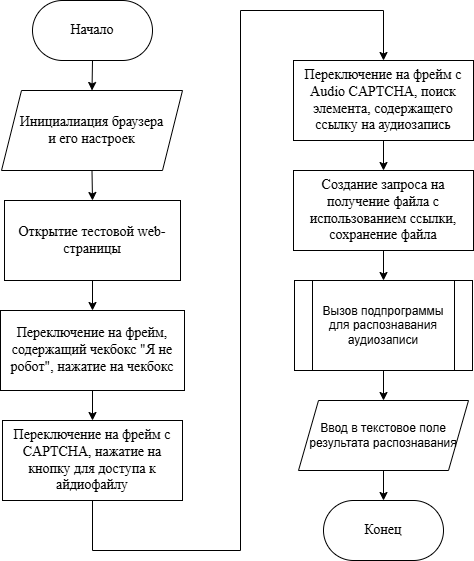
\includegraphics[width=0.6\linewidth]{imgs/audiocaptcha/captcha_solve.png}
    \caption{Блок-схема процесса прохождения Audio CAPTCHA.}
    \label{fig:audio-solver}
\end{figure}

Процесс обработки аудиофайла, полученного с web-страницы можно разделить на 
следующие этапы:

\begin{enumerate}
    \item преобразование полученного аудиофайла в другой формат, который является 
    подходящим для распознавания;
    \item распознавание речи в перекодированном файле;
    \item сохранение полученного результата распознавания для последующей вставки 
    в тектстовое поле.
\end{enumerate}

На первом этапе исходный файл всегда имеет формат mp3, которое не пригодно для 
распознавания с использованием SpeechRecognition, поскольку данный формат 
использует сжатие с потерями, поэтому исходный файл необходимо перекодировать в 
формат wav. Для перекодирования файла используется библиотека с открытым исходным 
кодом -- ffmpeg, которая предоставляет обширные возможности для работы с любыми 
мультимедиа файлами [9].

На следующем этапе создается объект для распознавания, который содержит 
перекодированный файл. Распознавание происходит с использованием Google Web 
Speech API, поскольку данный API обеспечивает более высокую точность 
распознавания среди прочих [10].

Результатом распознавания является текстовое сообщение, которое сохраняется для 
последующих действий в браузере.

Описанный алгоритм можно представить в виде следующей блок-схемы (рис.~
\ref{fig:recognize-audio}):

\begin{figure}[H]
    \centering
    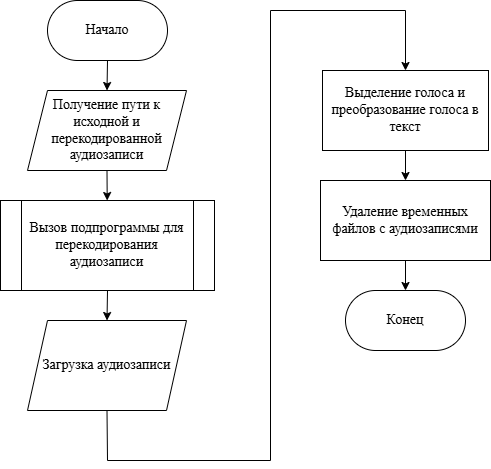
\includegraphics[width=0.6\linewidth]{
        imgs/audiocaptcha/recognize_audiocaptcha.png
    }
    \caption{Блок-схема процесса распознавания Audio CAPTCHA.}
    \label{fig:recognize-audio}
\end{figure}

\section{Автоматизация решения CAPTCHA в формате изображений}

\textbf{Выбор модели нейронной сети для обучения}

CAPTCHA в формате изображений широко используется для защиты ресурсов от 
автоматизированных ботов и может быть реализована несколькими способами. Как 
правило, такие CAPTCHA направлены на проверку способности пользователя 
распознавать и интерпретировать объекты на изображении. Наиболее распространены 
два варианта реализации (оба варианта реализации проиллюстрированы на рис.~
\ref{fig:example}):

\begin{enumerate}
    \item цельное изображение, содержащее несколько объектов, частично размытых 
    или искажённых, при этом изображение разбито на сетку 3×3 или 4×4. 
    Пользователю предлагается выбрать ячейки, содержащие объекты определённого 
    класса (например, автобусы или светофоры);
    \item составное изображение, сформированное из 9 или 12 отдельных фрагментов 
    (изображений), каждый из которых представляет собой независимое изображение 
    -- зачастую низкого качества, с наложением артефактов или шумов. Задача 
    пользователя -- выбрать те изображения, где присутствует нужный объект.
\end{enumerate}

\begin{figure}[!ht]
    \begin{minipage}[h]{0.49\linewidth}
        \center{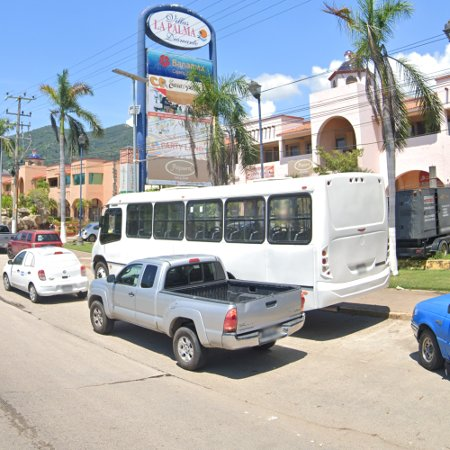
\includegraphics[width=1\linewidth]{imgs/imagecaptcha/6.jpg} \\ 
        а)}
    \end{minipage}
    \hfill
    \begin{minipage}[h]{0.49\linewidth}
        \center{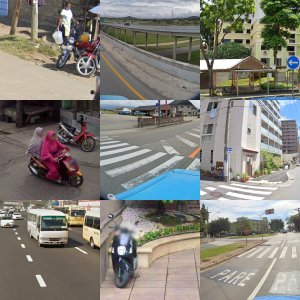
\includegraphics[width=1\linewidth]{imgs/imagecaptcha/8.jpg} \\ 
        б)}
    \end{minipage}
    \caption{Изображения CAPTCHA с размером сетки 3×3: а) -- цельное, б) -- 
    составное.}
    \label{fig:example}
\end{figure}
\vspace{-0.5cm}

Такие CAPTCHA требуют от системы автоматического анализа способности как к 
глобальному восприятию изображения, так и к локальной интерпретации его 
фрагментов. Соответственно, модель, предназначенная для решения данной задачи, 
должна поддерживать:

\begin{enumerate}
    \item классификацию объектов на уровне отдельных изображений (для CAPTCHA, 
    основанных на отдельных картинках в сетке);
    \item локализацию и сегментацию объектов с высокой точностью, чтобы 
    корректно определить границы объектов в пределах ячеек, особенно в случаях, 
    когда объект может частично заходить за границу между ячейками.
\end{enumerate}

Для решения этих задач были рассмотрены следующие современные архитектуры 
нейронных сетей:

\begin{enumerate}
    \item YOLO (You Only Look Once) -- однопроходная модель, объединяющая 
    классификацию и регрессию ограничивающих рамок в одной свёрточной 
    архитектуре. Отличается высокой скоростью и хорошей точностью~
    \cite{redmon2016yolov2, UltralyticsYOLOv8};
    \item Faster R-CNN -- двухступенчатая модель, в которой сначала генерируются 
    области предложений, а затем выполняется классификация и уточнение рамок. 
    Обладает высокой точностью, но уступает в скорости~\cite{ren2015fasterrcnn};
    \item DETR (DEtection TRansformer) -- основана на архитектуре трансформеров, 
    что позволяет эффективно моделировать глобальные взаимосвязи между объектами. 
    Подходит для задач с большим количеством контекстных зависимостей, но требует 
    больше ресурсов для обучения~\cite{carion2020detr}.
\end{enumerate}

Среди этих архитектур было принято решение использовать YOLOv8 по следующим 
причинам:

\begin{enumerate}
    \item высокая производительность: YOLOv8 показывает высокую скорость 
    обработки изображений без значительного ущерба для точности, что критично в 
    условиях, когда необходимо обрабатывать CAPTCHA в реальном времени~
    \cite{bochkovskiy2020yolov4};
    \item гибкость и масштабируемость: модель предоставляет множество 
    предобученных вариантов с различной глубиной и числом параметров (версии n, 
    s, m, l, x), что позволяет использовать как на слабых, так и на 
    производительных устройствах;
    \item широкая поддержка и документация: YOLOv8 имеет активное сообщество, 
    подробную документацию и регулярно обновляется, что значительно упрощает 
    интеграцию и адаптацию модели под пользовательские задачи;
    \item поддержка сегментации: в отличие от более ранних версий, YOLOv8 
    поддерживает не только детекцию, но и сегментацию объектов, что особенно 
    важно для задач, где необходимо точно определить область объекта внутри 
    изображения;
    \item дообучение на пользовательских данных: YOLOv8 позволяет эффективно 
    дообучать модель на собственных датасетах, что особенно важно при работе с 
    CAPTCHA-изображениями, содержащими специфические классы объектов и 
    нестандартные искажения.
\end{enumerate}

Кроме того, модель YOLOv8 была успешно протестирована в задачах, близких по 
структуре к CAPTCHA: детекции дорожных знаков, транспортных средств, пешеходов и 
других объектов в сложных условиях съёмки, что подтверждает её универсальность и 
применимость к рассматриваемой задаче.

Таким образом, YOLOv8 является наиболее сбалансированным выбором, обеспечивающим 
как точную классификацию, так и локализацию объектов в условиях ограниченных 
ресурсов и с возможностью адаптации под специфику визуальных CAPTCHA.

\section{Исследовательский вклад}

\textbf{Тестирование выбранной модели нейронной сети (text captcha)}

Как было установлено в предыдущих разделах, модель последовательного 
преобразования (Seq-to-Seq) продемонстрировала наилучшие результаты среди 
рассмотренных архитектур. Следующим этапом работы являлась оптимизация параметров 
модели, включая веса и коэффициенты регуляризации, с целью ускорения сходимости, 
минимизации риска переобучения и повышения точности распознавания целевых 
последовательностей.

Для проведения экспериментов исходный набор данных, содержащий 100 000 
изображений, был случайным образом перемешан и разделён на три подмножества: 
обучающее, тестовое и валидационное в соотношении 80:10:10. Обучающая выборка 
использовалась непосредственно для обучения модели, валидационная — для контроля 
качества процесса обучения на каждой эпохе, а тестовая — для окончательной 
оценки модели на данных, с которыми она ранее не сталкивалась. В качестве 
основных метрик качества модели использовались функция потерь (loss) и точность 
(accuracy), рассчитываемая для каждого символа последовательности.

В процессе многократного обучения были экспериментально определены оптимальное 
количество эпох и значения гиперпараметров, обеспечивающие эффективное снижение 
функции потерь до приемлемых значений. График сходимости функции потерь 
представлен на рис.~\ref{fig:loss}.

\begin{figure}[H]
    \centering
    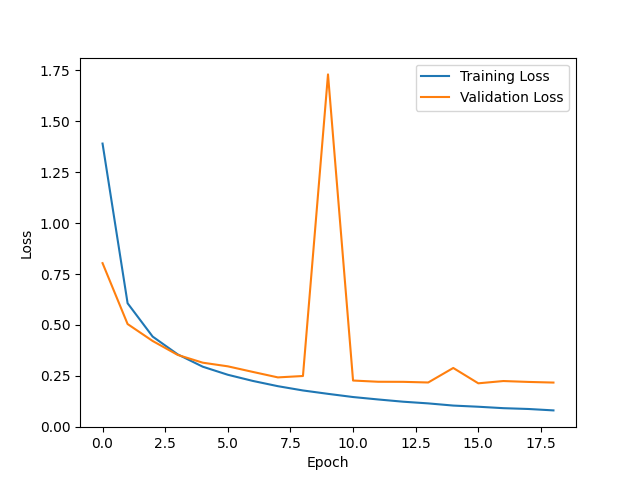
\includegraphics[width=0.8\linewidth]{imgs/textcaptcha/Model_loss.png}
    \caption{График изменения значений функции потерь в процессе обучения.}
    \label{fig:loss}
\end{figure}

Для предотвращения переобучения использовался механизм ранней остановки, согласно 
которому обучение прекращалось при отсутствии уменьшения значения функции потерь 
на валидационной выборке в течение трёх последовательных эпох. В данном 
эксперименте обучение завершилось на 18-й эпохе. На графике видно, что функция 
потерь стабилизировалась после 10 эпохе, поэтому 10 эпоха является балансом между 
точностью распознавания последовательностей и скоростью обучения модели.

Анализ графика сходимости функции потерь показывает наличие резкого увеличения её 
значения на 9-й эпохе, что может быть обусловлено следующими факторами:

\begin{enumerate}
    \item перемешивание данных перед каждой эпохой могло привести к образованию 
    несбалансированной выборки, содержащей значительное число сложных примеров.
    \item динамическое изменение скорости обучения, осуществляемое с помощью 
    механизма регулирования скорости обучения (learning rate scheduler), могло 
    повлиять на изменение функции потерь.
\end{enumerate}

Окончательная точность распознавания отдельных символов составила 0.9263.

После подбора оптимальных значений гиперпараметров модель была сохранена и 
протестирована на валидационной выборке. Точность распознавания 
последовательностей различной длины представлена в таблице~\ref{tab:probability}.

\begin{table}[H]
    \centering
    \caption{Точность предсказаний для последовательностей различной длины.}
    \begin{tabular}{|l|l|}
        \hline
        Длина последовательности & Точность распознавания \\
        \hline
        4 символа & 0.9305 \\
        \hline
        5 символов & 0.7450 \\
        \hline
        6 символов & 0.4575 \\
        \hline
        7 символов & 0.1915 \\
        \hline
    \end{tabular}
    \label{tab:probability}
\end{table}

Также была построена матрица ошибок, позволяющая проанализировать частоту и 
характер ошибок модели при классификации различных классов. Данная матрица 
приведена на рис.~\ref{fig:cm}.

\begin{figure}[H]
    \centering
    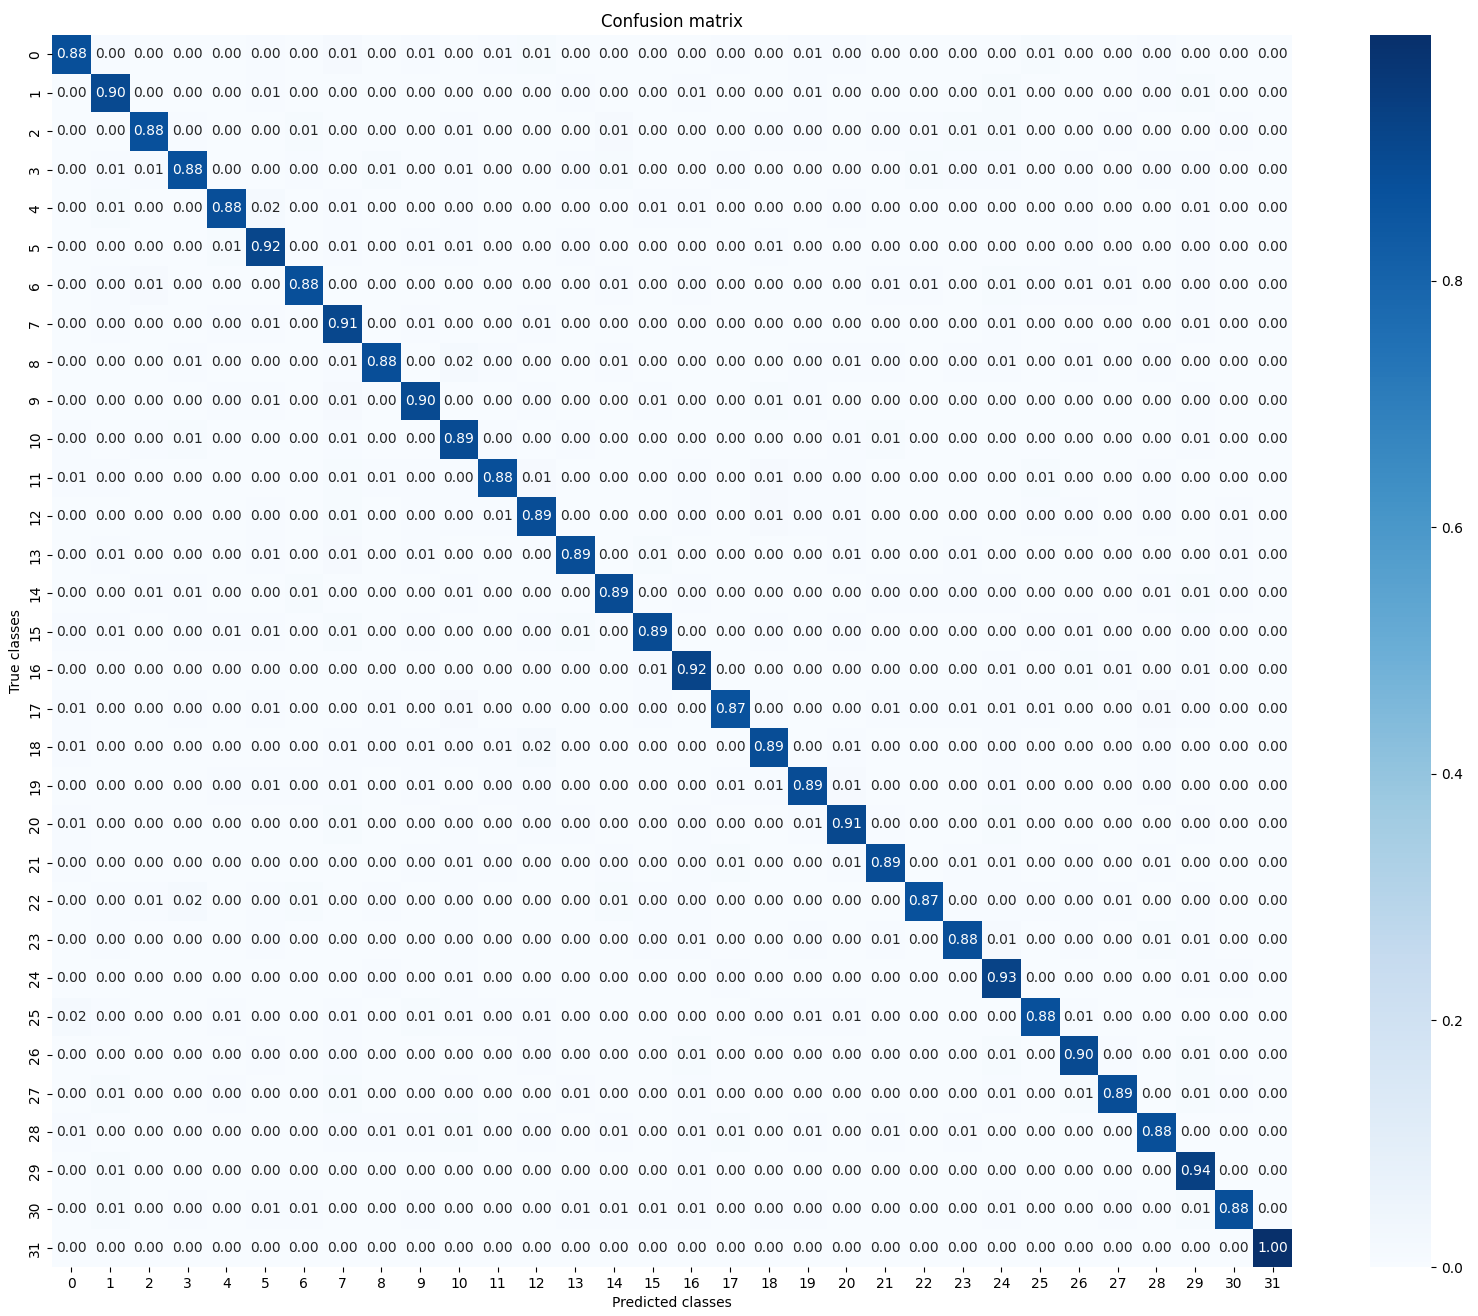
\includegraphics[width=1\linewidth]{imgs/textcaptcha/Confusion_matrix.png}
    \caption{Матрица ошибок для обученной модели.}
    \label{fig:cm}
\end{figure}

Анализ полученных результатов показывает, что точность распознавания 
последовательностей значительной длины остаётся относительно низкой. Это можно 
объяснить высокой зависимостью модели Seq-to-Seq от объёма обучающих данных: для 
эффективного обобщения признаков, извлекаемых из изображений, требуется 
значительное количество примеров. Следовательно, увеличение размера обучающего 
набора данных потенциально может способствовать повышению точности модели, 
однако это также накладывает дополнительные требования к вычислительным ресурсам, 
необходимым для её обучения.

\textbf{Тестирование модели (image captcha)}

После завершения обучения модель была протестирована на реальных CAPTCHA, 
собранных с помощью автоматического парсера, реализованного на базе библиотеки 
Selenium. Тестирование проводилось в автоматическом режиме, имитируя реальные 
действия пользователя в браузере, что позволило оценить работоспособность системы 
в условиях, приближенных к реальной эксплуатации.

Сценарий тестирования предусматривал выполнение следующих шагов:

\begin{enumerate}
    \item автоматический переход к странице с CAPTCHA и активация чекбокса <<Я не 
    робот>>;
    \item извлечение изображения CAPTCHA (включая структуру сетки и текст 
    задания);
    \item определение целевого объекта из текста задания (например, «выберите все 
    изображения с автобусами»);
    \item разбиение изображения CAPTCHA на ячейки (в зависимости от размера сетки 
    -- 3×3 или 4×4);
    \item применение обученной модели для сегментации и классификации каждого 
    изображения или фрагмента;
    \item определение ячеек, содержащих нужный класс, и программная симуляция 
    кликов по ним;
    \item повторная попытка прохождения CAPTCHA в случае, если результат оказался 
    некорректным (что также фиксировалось в логах).
\end{enumerate}

Тестирование было организовано в виде цикла, позволяющего автоматически проходить 
CAPTCHA до тех пор, пока не будет достигнут положительный результат. Это 
позволило зафиксировать частоту ошибок модели и определить случаи, в которых 
требуются дообучение или оптимизация.

Рабочий процесс тестирования и взаимодействия модели с CAPTCHA представлен на 
блок-схеме ниже.

\begin{figure}[H]
    \centering
    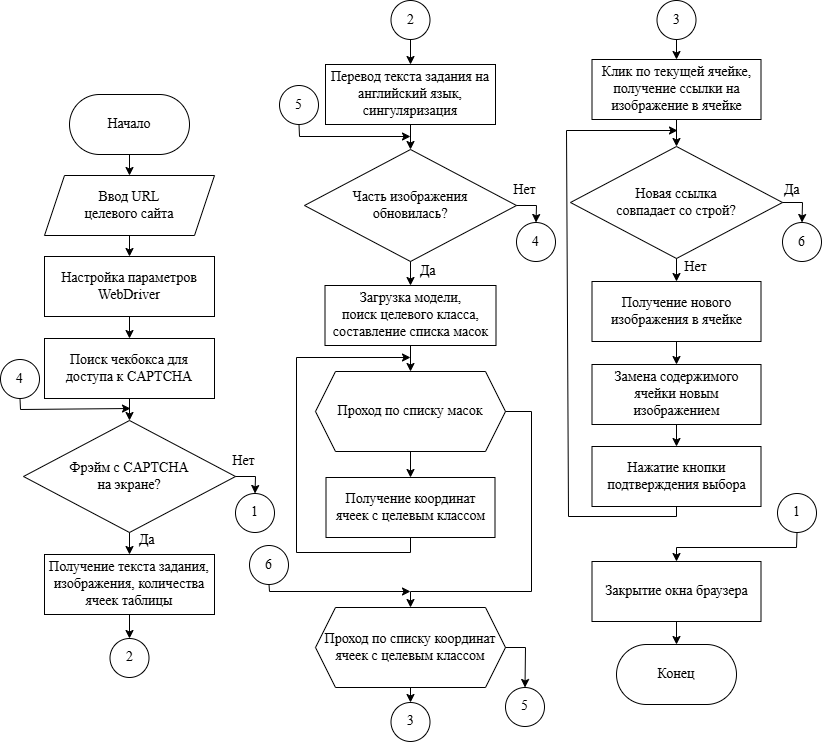
\includegraphics[width=1\textwidth]{imgs/imagecaptcha/solve_captcha_flow.png}
    \caption{Блок-схема процесса прохождения CAPTCHA.}
    \label{fig:solve-captcha}
\end{figure}
\vspace{-0.5cm}

Полученные данные используются для последующего анализа качества модели и 
корректировки процесса обучения. Основное внимание при анализе будет уделено 
типам ошибок, сложности распознаваемых объектов и влиянию качества исходного 
изображения на точность сегментации.

\textbf{Обучение модели}

В качестве основной архитектуры была выбрана модель YOLOv8m-seg, поддерживающая 
сегментацию объектов. Она представляет собой сбалансированное решение между 
качеством распознавания, производительностью и требованиями к аппаратному 
обеспечению. Благодаря своей универсальности, модель подходит как для задач 
классификации, так и для задач детектирования и сегментации, что особенно важно 
при работе с CAPTCHA, содержащими зашумлённые или плохо различимые объекты.

Преимущества YOLOv8m-seg заключаются в следующем:

\begin{enumerate}
    \item наличие встроенной поддержки сегментации объектов, что особенно важно 
    при необходимости выделения фрагментов изображений;
    \item возможность использования предобученных весов, сокращающих время на 
    обучение и повышающих стартовую точность;
    \item высокая скорость инференса по сравнению с другими моделями сегментации 
    (например, Mask R-CNN или DETR);
    \item встроенные средства аугментации (изменения яркости, повороты, 
    масштабирование и пр.);
    \item удобный интерфейс через библиотеку ultralytics, позволяющий быстро 
    запускать обучение, логировать метрики и визуализировать результаты;
    \item полная совместимость с аннотациями в формате YOLO, полученными из CVAT.
\end{enumerate}

Перед запуском обучения структура данных была организована в соответствии с 
требованиями YOLOv8: директории train и val содержали соответствующие изображения 
и файлы разметки, а в .yaml файле конфигурации были указаны пути к выборкам и 
список классов.

Обучение проводилось на 35 эпохах при размере изображений 640×640 пикселей и 
размере батча 8. Использование предобученных весов позволило достичь стабильного 
снижения функции потерь с первых эпох, а встроенные механизмы аугментации 
способствовали улучшению обобщающей способности модели.

Результаты обучения отслеживались по ключевым метрикам (IoU, Precision, Recall, 
Loss), которые визуализировались автоматически. Примеры графиков с результатами 
обучения приведены ниже:

\begin{figure}[H]
    \centering
    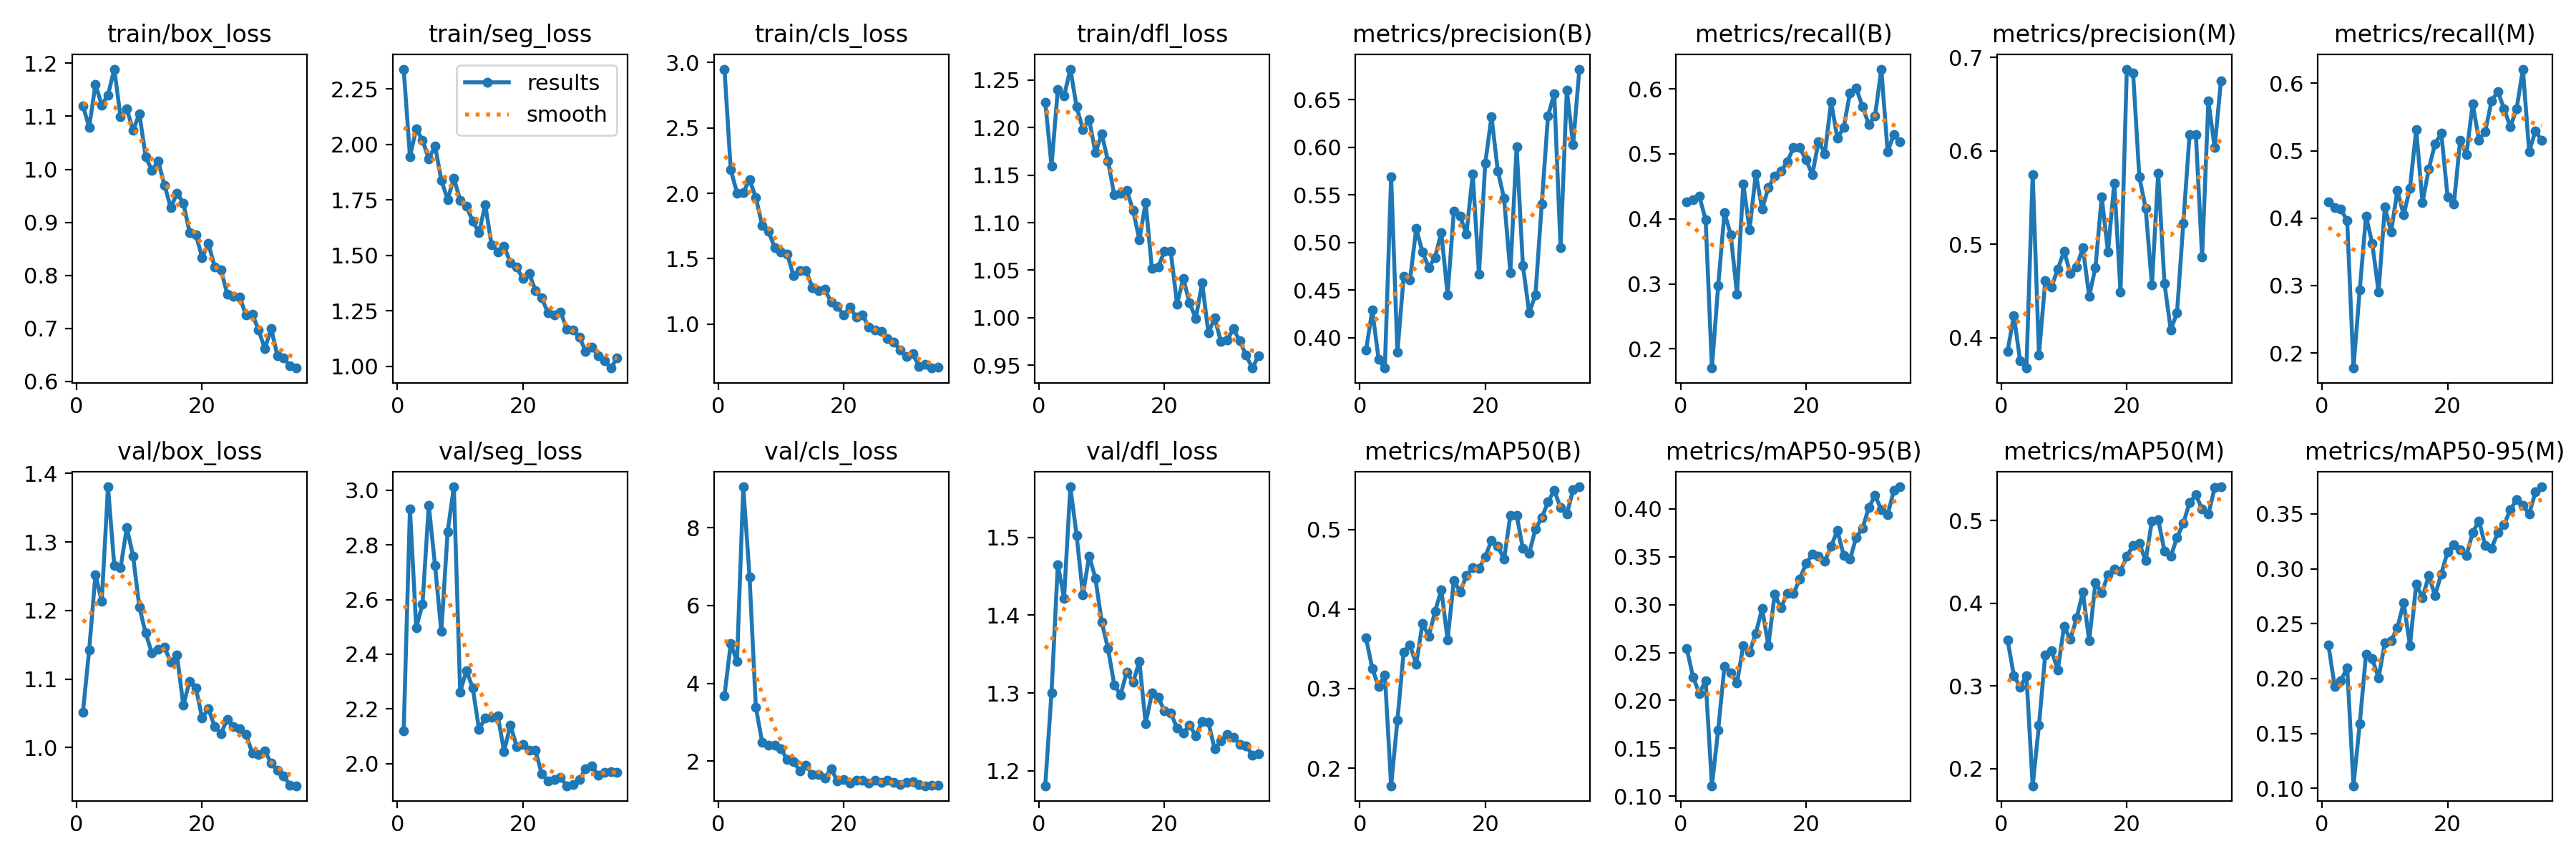
\includegraphics[width=1\linewidth]{imgs/imagecaptcha/results.png}
    \caption{Изменение ключевых метрик в процессе обучения.}
    \label{fig:metrics}
\end{figure}
\vspace{-0.5cm}

Также, была построена нормализованная матрица ошибок для определения точности 
предсказания необходимых классов на валидационной выборке, которая представлена 
на рис.~\ref{fig:confusion}.

\begin{figure}[H]
    \centering
    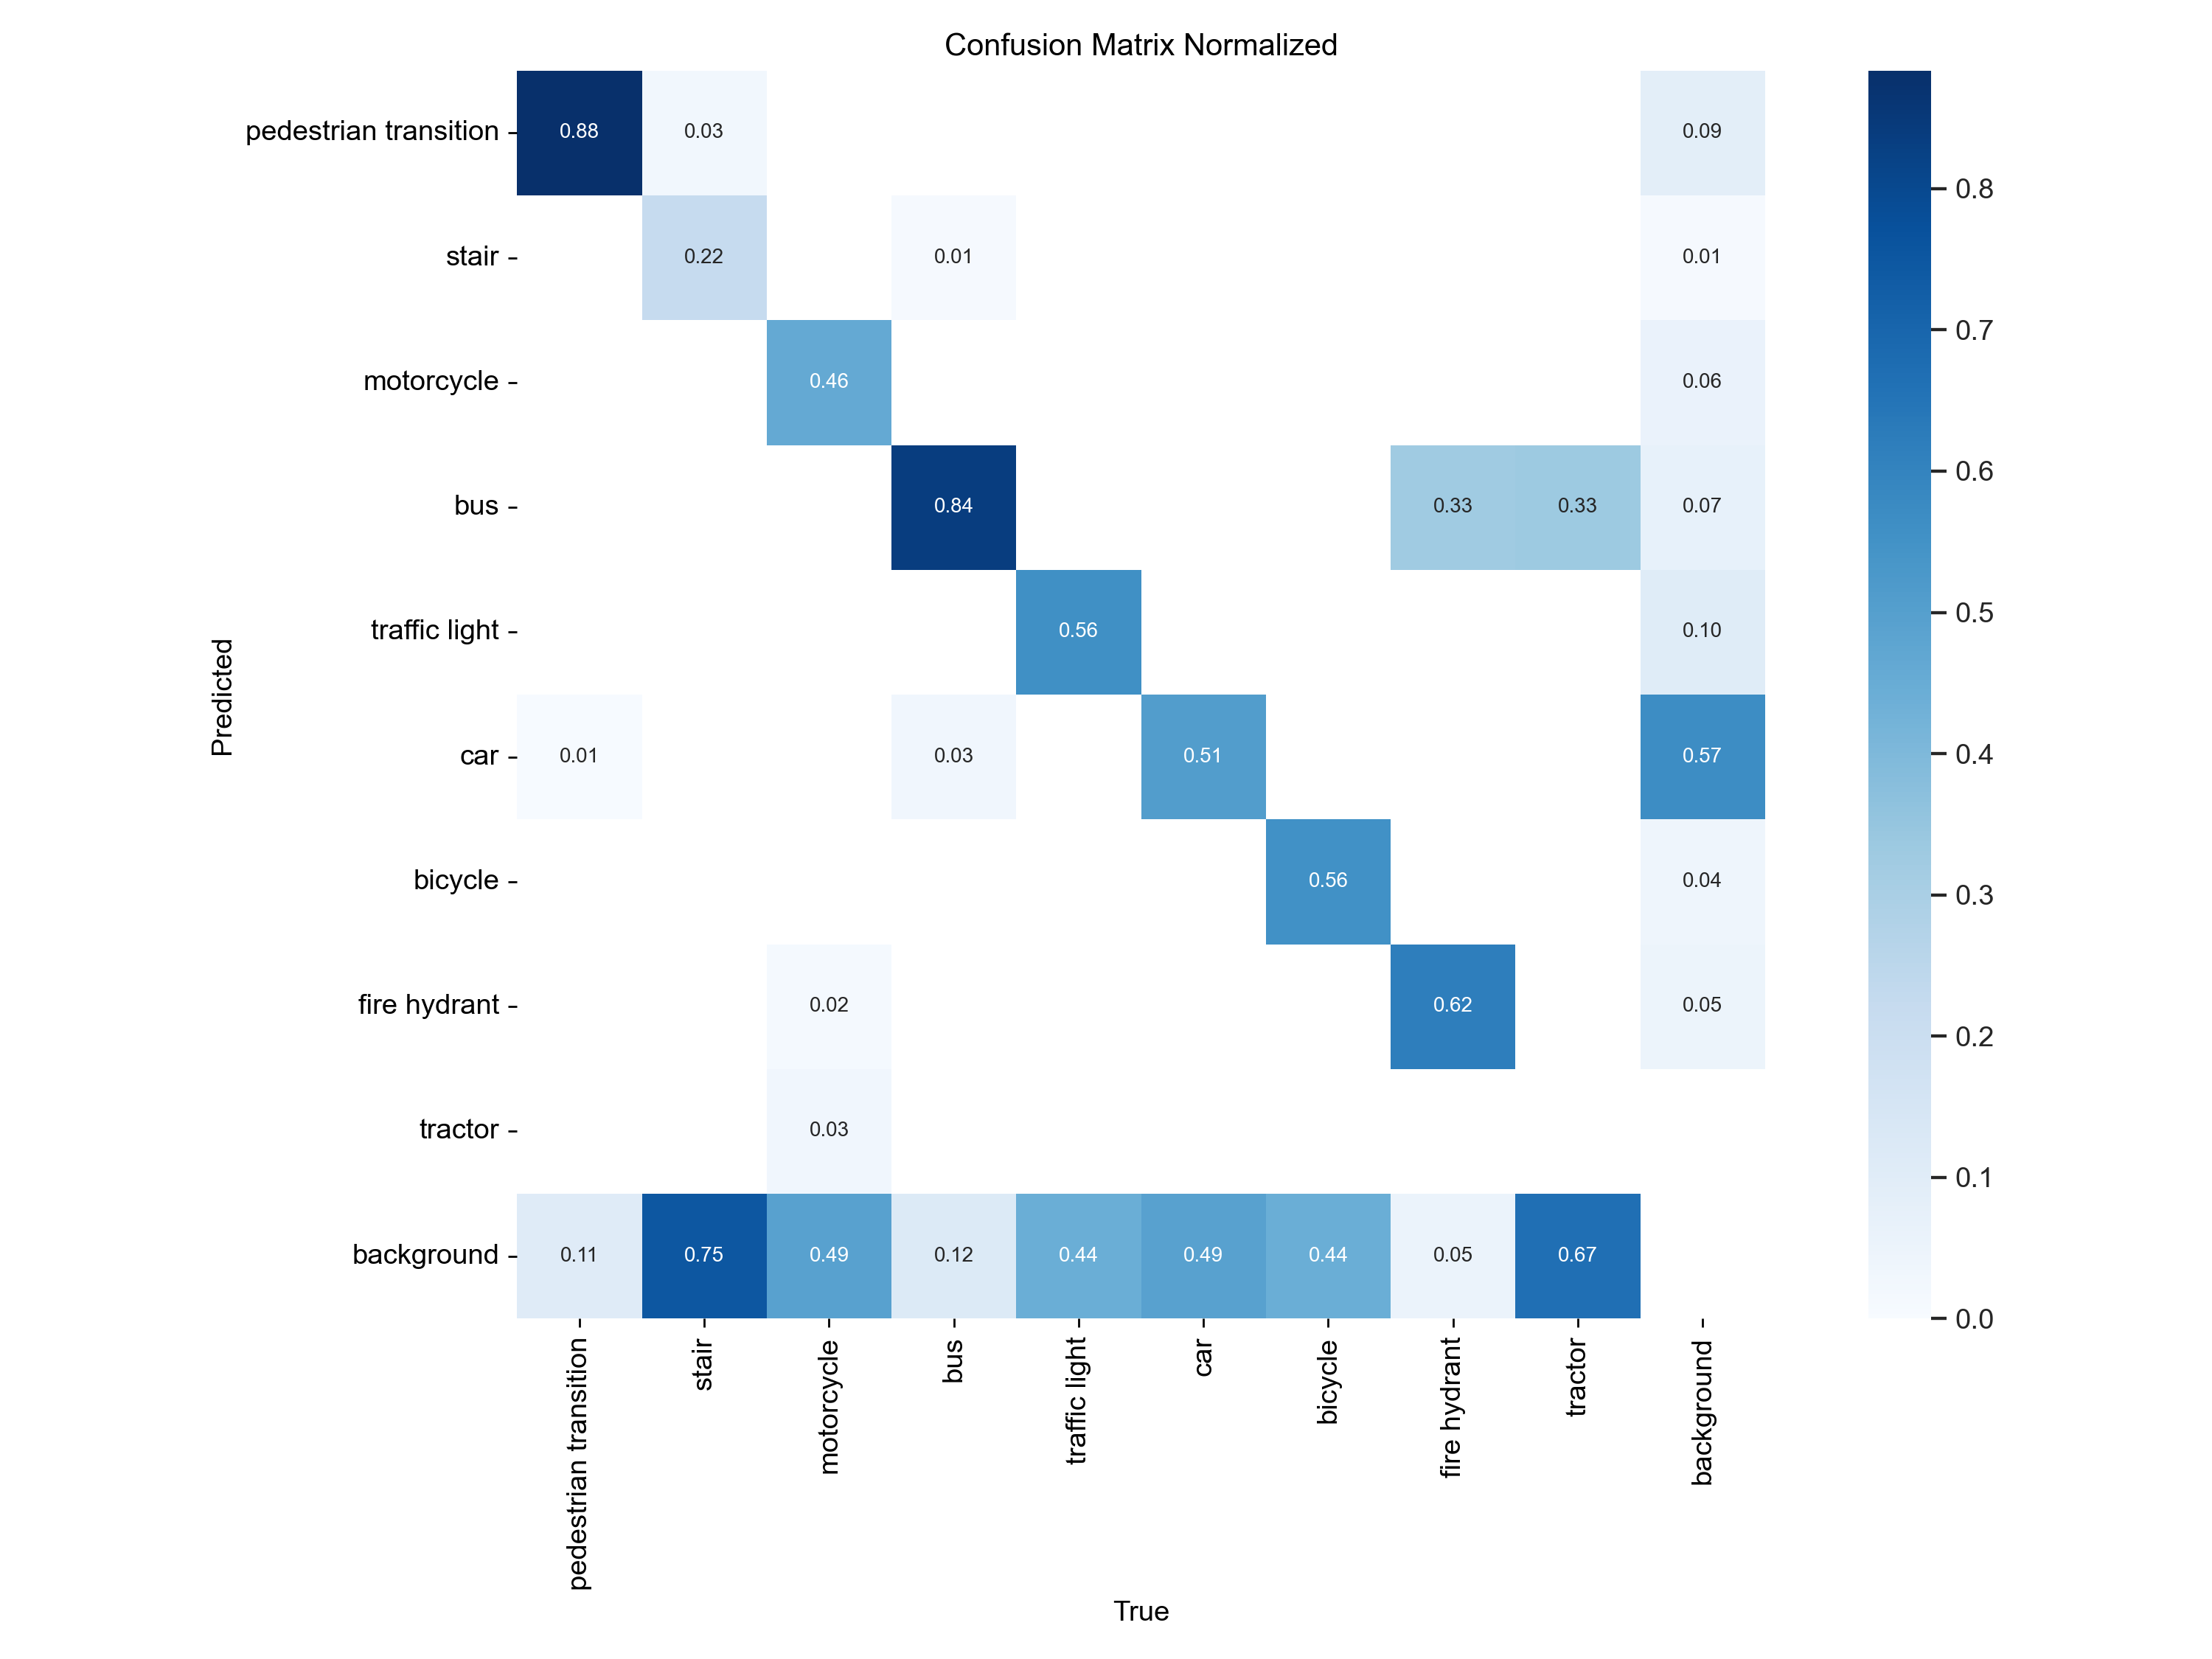
\includegraphics[width=1\linewidth]{
        imgs/imagecaptcha/confusion_matrix_normalized.png
    }
    \caption{Матрица ошибок для изображений валидационной выборки.}
    \label{fig:confusion}
\end{figure}
\vspace{-0.5cm}
\chapter{Обсуждение, выводы и перспективы развития}

\section{Анализ надежности и уязвимостей решений}

\section{Ограничения проведенных экспериментов}

\section{Перспективные направления}



\newpage
\addcontentsline{toc}{chapter}{СПИСОК ИСПОЛЬЗОВАННОЙ ЛИТЕРАТУРЫ}
\printbibliography[title={СПИСОК ИСПОЛЬЗОВАННОЙ ЛИТЕРАТУРЫ}]

\appendix
\newpage
\chapter*{\begin{flushright}\raggedleft\label{appendix1}Приложение 1\end{flushright}}
\phantomsection\addcontentsline{toc}{chapter}{ПРИЛОЖЕНИЕ 1}
\vspace{-1.75cm}

\begin{center}
\label{code:appendix}Текст программ для автоматизации решения аудио CAPTCHA
\end{center}

\begin{code}
    \captionof{listing}{\label{code:audiocaptcha}Исходный код расшифровки Audio CAPTCHA}
    \vspace{-1cm}
    \inputminted{python}{code/audiocaptcha/audiocaptcha.py}
\end{code}

\begin{code}
    \captionof{listing}{\label{code:audiocaptcha-solve}Исходный код автоматизированного решения Audio CAPTCHA}
    \vspace{-1cm}
    \inputminted{python}{code/audiocaptcha/audiocaptcha_solve.py}
\end{code}

\appendix
\newpage
\chapter*{\begin{flushright}\raggedleft\label{appendix2}Приложение 2\end{flushright}}
\phantomsection\addcontentsline{toc}{chapter}{ПРИЛОЖЕНИЕ 2}
\vspace{-1.75cm}

\begin{center}
\label{code:appendix2}Текст программ для автоматизации решения текстовых CAPTCHA
\end{center}

\begin{code}
    \captionof{listing}{\label{code:gen-dataset}Исходный код генератора синтетических текстовых CAPTCHA}
    \vspace{-1cm}
    \inputminted{python}{code/textcaptcha/gen-dataset.py}
\end{code}

\begin{code}
    \captionof{listing}{\label{code:preprocessing}Исходный код для предобработки изображений датасета с текстовыми CAPTCHA}
    \vspace{-1cm}
    \inputminted{python}{code/textcaptcha/preprocessing.py}
\end{code}

\begin{code}
    \captionof{listing}{\label{code:tf-dataset}Исходный код для создания датасета текстовых CAPTCHA в формате тензоров}
    \vspace{-1cm}
    \inputminted{python}{code/textcaptcha/tf-dataset.py}
\end{code}

\begin{code}
    \captionof{listing}{\label{code:crnn}Исходный код CRNN модели}
    \vspace{-1cm}
    \inputminted{python}{code/textcaptcha/crnn.py}
\end{code}

\begin{code}
    \captionof{listing}{\label{code:seq2seq}Исходный код Seq2Seq модели}
    \vspace{-1cm}
    \inputminted{python}{code/textcaptcha/seq-to-seq.py}
\end{code}

\begin{code}
    \captionof{listing}{\label{code:test-model}Исходный код тестирования Seq2Seq модели}
    \vspace{-1cm}
    \inputminted{python}{code/textcaptcha/test.py}
\end{code}

\appendix
\newpage
\chapter*{\begin{flushright}\raggedleft\label{appendix3}Приложение 3\end{flushright}}
\phantomsection\addcontentsline{toc}{chapter}{ПРИЛОЖЕНИЕ 3}
\vspace{-1.75cm}

\begin{center}
\label{code:appendix3}Текст программ для автоматизации решения графических CAPTCHA
\end{center}

\begin{code}
    \captionof{listing}{\label{code:get-captcha}Исходный код получения графических CAPTCHA с целевого сайта}
    \vspace{-1cm}
    \inputminted{python}{code/imagecaptcha/get_captcha.py}
\end{code}

\begin{code}
    \captionof{listing}{\label{code:recognize}Исходный код дообучения модели на датасете с графическими CAPTCHA}
    \vspace{-1cm}
    \inputminted{python}{code/imagecaptcha/recognize_objects.py}
\end{code}

\begin{code}
    \captionof{listing}{\label{code:solve-captcha}Исходный код автоматизированного решения графических CAPTCHA}
    \vspace{-1cm}
    \inputminted{python}{code/imagecaptcha/solve_captcha.py}
\end{code}

\makelastpage
\end{document}
